\documentclass[a4paper, article, 11pt, oneside]{memoir}
% General packages
\usepackage[T1]{fontenc} 
\usepackage{lmodern}
\usepackage[utf8]{inputenc}
\usepackage[english]{babel}
\usepackage[final]{microtype}
\usepackage{multicol}
\usepackage{amssymb}
\usepackage{adjustbox}
\usepackage{amsmath}
\usepackage{siunitx}
\usepackage{cancel}
\usepackage[normalem]{ulem}
\usepackage{ragged2e}
\usepackage{geometry}
\usepackage{graphicx}
\usepackage{float}
\usepackage{tabularx}
\usepackage{lipsum}
\usepackage{wrapfig}
\usepackage{tikz, pgfplots}
\usetikzlibrary{er}
\pgfplotsset{compat=1.16}
\usepackage{notoccite}
\usepackage{pythonhighlight}
\usepackage{scalerel}
\usepackage[hyphens]{url}
\usepackage{ifthen}
\usepackage{csquotes}
\usepackage[breaklinks]{hyperref}
\usepackage{listings}
\hypersetup{
    colorlinks=true,
    linkcolor=black,
    filecolor=magenta,      
    urlcolor=cyan,
}
\geometry{
 top = 25mm,
 left = 30mm,
 right = 30mm,
 bottom = 25mm,}

 %lstlisting setup
\lstset
{
    basicstyle=\footnotesize,
    numbers=left,
    stepnumber=1,
    showstringspaces=false,
    tabsize=1,
    breaklines=true,
    breakatwhitespace=false,
}
%Python env
\usepackage{pythonhighlight}
\definecolor{jet_orange}{HTML}{CC7832}
\definecolor{jet_green}{HTML}{6A8759}
\colorlet{stringcolour}{jet_green}
\colorlet{keywordcolour}{jet_orange}
\colorlet{exceptioncolour}{yellow!50!red}
\colorlet{commandcolour}{blue!60!black}
\colorlet{literatecolour}{magenta!90!black}
\colorlet{promptcolour}{green!50!black}
\colorlet{specmethodcolour}{violet}

\title{Data report on the methylization of cell-free DNA}

\author{Daniel, Thomas \& Hans-Henrik}
\date{\today}

\begin{document}

\maketitle
\tableofcontents*
\newpage
\chapter{Quick overview of repo}
This is a quick overview of the structure of the repo.
We have divided everything into various folders, we highly recommend reading the introduction here in order to understand the purpose of the project. 
Starting from the top we have the "figures" folder. This and certain other folders contain 3 subfolders for the various areas of our project, each of these subfolders contain more folders in which various figures and tables relating to the project can be found. 
The "Model" folder contains joblibs of our models created by the scripts and notebooks in this repo.
The "notebooks" folder contains jupyter notebooks as well a R markdowns for various processes going from creating to models to organizing our data.
This is closely related to the "Scripts" folder this contains scripts of various kinds, do note that while some notebooks do have script counterparts not all do, and not all scripts have a notebook. 
The data is split across 3 folders. The zip files are found in "zip\_files" we extracted this into the "raw\_data" folder. Which also includes combined tables.
The "processed\_data" is the data after being normalized, this is primarily the data we used in our various processes.
The "tex" folder contains all of our LaTeX related items.

\chapter{Introduction}
In this project we will be looking at attempting to implement a model to predict, based on data from blood analysis, whether a given person potentially has cancer.
The method in which we will be doing this, is by looking at methylized/unmethylized cell-free dna in peoples blood, specifically the fragmentation patterns.
This is preferable to other methods, since it is both less invasive, and less expensive.

The data we will be looking at in this project, has been provided to us by Søren Bessenbacher, and contains information regarding fragmentation patterns for approximately 230 people diagnosed with cancer, and 230 people as a control group.

\newpage
\chapter{The data}
\begin{figure}[H]
	\centering
	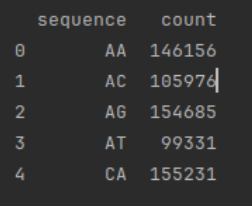
\includegraphics[width=0.7\linewidth]{../figures/data_example}
	\caption{An example of the data}
	\label{fig:data0}
\end{figure}

In the first column we have the k-mer, in this specific figure it is a 2-mer, and in the second column we have the count of that specific sequence. In addition to the control and the test samples, we also have a background file, which details the total number of combinations of sequences.

\newpage
\chapter{Normalizing the data}
The raw data with just the counts, would likely not work, thus we want to normalize the data. The way in which we do this is by taking the sum of all the counts in a given file, and then dividing each count cell by this sum, thus giving us a ratio of the data. The way in which we've programmed this can be found in the \textit{scripts/} folder of this repository, called \textit{normalize\_data.sh}. This script does as previosly mentioned and writes the ratios into a new file, which can be found in the folder \textit{processed\_data/normalized\_data}. We then combine all these matrices into a single matrix with a R-script, which can also be found in the \textit{scripts/}. The new file can be found in the the \textit{processed\_data/combined\_data/}.

\section{Normalizing with the background}
In order to see the ratios of the samples compared to the potential ratios of the region in question, one can also normalize with the background file found in each k-mer folder. The way in which we approached this, was as previous by taking the sum of each count column, and then in addition we divide each cell in each sample with their respective background ratio. We did this with the \textit{normalize\_data\_with\_background.sh} file, which can be found in the \textit{scripts/} folder.

\section{PCA}
To make the data approachable, it would be desirable to transform the data into a smaller dimension, we do this by using \textit{Principal Component Analysis}. The way in which do this is by using the function from \textit{sklearn} called PCA. An example could be:
\begin{python}
from sklearn.decomposition import PCA
...
def pca_fit(data):
    pca = PCA(n_components=2)
    pca.fit(data)
    data_pca = pca.transform(data)

    return data_pca
...
\end{python}

\newpage
\chapter{Data exploration}
Now that the data has been normalized, we thought it natural to explore the data, and see if we could find something. The first thing we thought of was using \textit{clustering}. We thought of using \textit{k-means clustering}, and again we used the function \textit{sklearn}. One can see an example of how we implemented this:

\begin{python}
from sklearn.cluster import KMeans
...
def kmeans_cluster(data, n_clusters):
    kmeans = KMeans(n_clusters=n_clusters)
    kmeans.fit(data)
    y_kmeans = kmeans.predict(data)
    plt.scatter(data[:, 0], data[:, 1], c=y_kmeans, s=50, cmap='viridis')
    centers = kmeans.cluster_centers_
    plt.scatter(centers[:, 0], centers[:, 1], c='black', s=200, alpha=0.5)
...
\end{python}

One can also see an example of the resulting plot from taking the \textit{combined\_2mers} from the folder \textit{processed\_data/combined\_data/with\_background} here:

\begin{figure}[H]
	\centering
	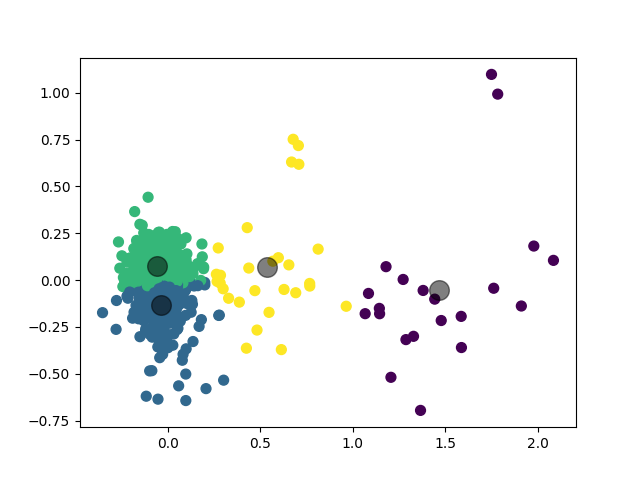
\includegraphics[width=0.7\linewidth]{../../figures/exploration/with_background/combined_2mers.png}
	\caption{A k-means clustering of the combined 2-mers file}
	\label{fig:kmeans0}
\end{figure}

Since we have; methylated/unmethylated, cancer/healthy. Which would result in four groupings of the data. We chose to make 4 clusters of the data.

The figure above is for our data normalized with the background, we have also looked into how the clusters look just normalizing each sample individually by looking at the ratios within the sample.

\begin{figure}[H]
	\centering
	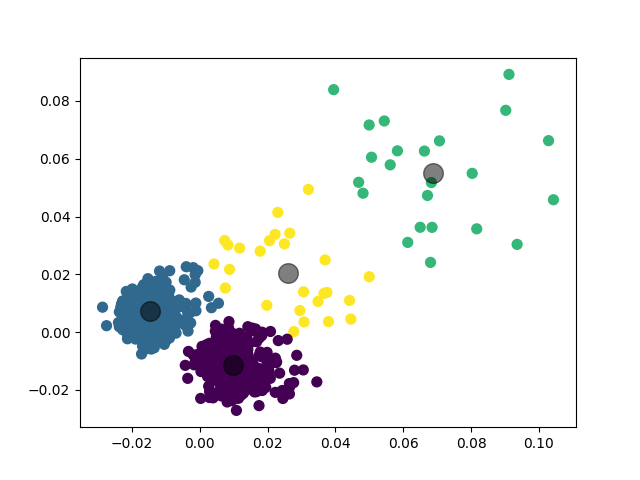
\includegraphics[width=0.7\linewidth]{../../figures/exploration/without_background/combined_2mers.png}
	\caption{A k-means clustering of the combined 2-mers file without proper normalization}
	\label{fig:kmeans1}
\end{figure}

As you can see the divide between clusters is somewhat more clear here, however the eventual goal is distinguishing our cases from controls is more difficult using this form of normalization.

\section{Even and Odd}
In order to test our normalization we had the data split into only taking the even/odd lines from each sample, therefore meaning that there should be a noticeable difference between odds and evens despite both being either methylated or unmethylated. To make this process more clear we focused purely on the controls. 

Unlike before where we were primarily interested in just seeing whether these clusters just existed, now we are interested in if we are getting 2 distinct clusters for our 4 groups. 

\begin{figure}[H]
	\centering
	\includegraphics[width=0.7\linewidth]{../../figures/exploration/all_healthy/all_healthy.png}
	\caption{A PCA plot of the 4 groups}
	\label{fig:allhealthy0}
\end{figure}

Here we are getting 1 large cluster although we are seeing that we are getting close to having 2 separate clusters. There is however 1 very clear outlier that may be affecting the PCA since one of the 2 components we are plotting may just be the variation caused by this outlier. Therefore we removed it and did the same plot again

\begin{figure}[H]
	\centering
	\includegraphics[width=0.7\linewidth]{../../figures/exploration/all_healthy/all_healthy_outlier_removed.png}
	\caption{A PCA plot of the 4 groups with the outlier removed}
	\label{fig:allhealthy1}
\end{figure}

As you can see this made the expected 2 clusters more distinct however there is still a large amount of overlap. We were not able to improve on this using only 2 principal components, although as we will detail later on we were able to clearly distinguish the 2 clusters using more principal components. 
For the sake of clarity we also looked into what this plot would look like without any form of normalization and just looking at the raw data.

\begin{figure}[H]
	\centering
	\includegraphics[width=0.7\linewidth]{../../figures/exploration/all_healthy/all_healthy_outlier_removed_raw.png}
	\caption{A PCA plot of the 4 groups with the outlier removed without normalization}
	\label{fig:allhealthy2}
\end{figure}

Much like in our initial exploration we can can see a more clear methylated/unmethylated divide. However, it is becoming more apparent why we need to normalize as there is a large amount of variance in the values of our principal components, making a later distinguishment of controls against cases more difficult 
\newpage
\chapter{Models}
We will make 2 models where the output of one is the input of the other. The first of these models determines the probability of a sample being either methylated or unmethylated. The second model determines based on those probabilities whether it comes from someone with a tumor or without. 
\section{Methylation  classification model}
This is the first proper step in the creation of the model that should be able to predict whether a given person may have a tumor based on blood analysis.

This first step is the creation of a \textit{binary classification model} to determine whether we are looking at a methylated or unmethylated region. We decided that a \textit{logistic regression} using \textit{L1 normalization (LASSO)} should be a good classifier. We used the same PCA data as in previous chapters to train and test the model. We decided that training on even and testing on odd should be adequate. Using \textit{SKlearn} we created the following code to create, train and test the model.

We end up with 100\% accuracy in our prediction of methylated and unmethylated, while this is regularly a red flag we do not find it too surprising as even just with 2 principal components we could almost separate methylated and unmethylated into 2 distinct clusters. Here is a graph showing the values of the coefficients for the different principal components.

With a good classifier for methylated and unmethylated set up we moved on to the next model.
\section{Tumor classification model}
In the previous model we trained on all healthy samples, now we are training on only half. We are now also testing on non-healthy patients, this should ideally give high confidence in predictions for healthy samples and lower confidence in predictions for non-healthy samples. The main idea with the model is to find where the confidence cutoff should be for both methylated and unmethylated such that we obtain the best model.


\newpage
\chapter{Conclusion}
Overall the straight model proved to be more effective though not by much, and we were not really able to get a high enough AUC for this to be a viable method for predicting cancer diagnosis. However, we have seen that there is a possibly a different model that is able to pick up the signals from the cancer samples better than the models we created. As such we would say that to some degree this project has been a success, and that more iteration in this space would potentially lead to a more accurate model.
\end{document}
